\documentclass[]{article}
\usepackage{lmodern}
\usepackage{amssymb,amsmath}
\usepackage{ifxetex,ifluatex}
\usepackage{fixltx2e} % provides \textsubscript
\ifnum 0\ifxetex 1\fi\ifluatex 1\fi=0 % if pdftex
  \usepackage[T1]{fontenc}
  \usepackage[utf8]{inputenc}
\else % if luatex or xelatex
  \ifxetex
    \usepackage{mathspec}
  \else
    \usepackage{fontspec}
  \fi
  \defaultfontfeatures{Ligatures=TeX,Scale=MatchLowercase}
\fi
% use upquote if available, for straight quotes in verbatim environments
\IfFileExists{upquote.sty}{\usepackage{upquote}}{}
% use microtype if available
\IfFileExists{microtype.sty}{%
\usepackage{microtype}
\UseMicrotypeSet[protrusion]{basicmath} % disable protrusion for tt fonts
}{}
\usepackage[margin=1in]{geometry}
\usepackage{hyperref}
\hypersetup{unicode=true,
            pdftitle={HW},
            pdfauthor={Amin Yakubu},
            pdfborder={0 0 0},
            breaklinks=true}
\urlstyle{same}  % don't use monospace font for urls
\usepackage{color}
\usepackage{fancyvrb}
\newcommand{\VerbBar}{|}
\newcommand{\VERB}{\Verb[commandchars=\\\{\}]}
\DefineVerbatimEnvironment{Highlighting}{Verbatim}{commandchars=\\\{\}}
% Add ',fontsize=\small' for more characters per line
\usepackage{framed}
\definecolor{shadecolor}{RGB}{248,248,248}
\newenvironment{Shaded}{\begin{snugshade}}{\end{snugshade}}
\newcommand{\KeywordTok}[1]{\textcolor[rgb]{0.13,0.29,0.53}{\textbf{#1}}}
\newcommand{\DataTypeTok}[1]{\textcolor[rgb]{0.13,0.29,0.53}{#1}}
\newcommand{\DecValTok}[1]{\textcolor[rgb]{0.00,0.00,0.81}{#1}}
\newcommand{\BaseNTok}[1]{\textcolor[rgb]{0.00,0.00,0.81}{#1}}
\newcommand{\FloatTok}[1]{\textcolor[rgb]{0.00,0.00,0.81}{#1}}
\newcommand{\ConstantTok}[1]{\textcolor[rgb]{0.00,0.00,0.00}{#1}}
\newcommand{\CharTok}[1]{\textcolor[rgb]{0.31,0.60,0.02}{#1}}
\newcommand{\SpecialCharTok}[1]{\textcolor[rgb]{0.00,0.00,0.00}{#1}}
\newcommand{\StringTok}[1]{\textcolor[rgb]{0.31,0.60,0.02}{#1}}
\newcommand{\VerbatimStringTok}[1]{\textcolor[rgb]{0.31,0.60,0.02}{#1}}
\newcommand{\SpecialStringTok}[1]{\textcolor[rgb]{0.31,0.60,0.02}{#1}}
\newcommand{\ImportTok}[1]{#1}
\newcommand{\CommentTok}[1]{\textcolor[rgb]{0.56,0.35,0.01}{\textit{#1}}}
\newcommand{\DocumentationTok}[1]{\textcolor[rgb]{0.56,0.35,0.01}{\textbf{\textit{#1}}}}
\newcommand{\AnnotationTok}[1]{\textcolor[rgb]{0.56,0.35,0.01}{\textbf{\textit{#1}}}}
\newcommand{\CommentVarTok}[1]{\textcolor[rgb]{0.56,0.35,0.01}{\textbf{\textit{#1}}}}
\newcommand{\OtherTok}[1]{\textcolor[rgb]{0.56,0.35,0.01}{#1}}
\newcommand{\FunctionTok}[1]{\textcolor[rgb]{0.00,0.00,0.00}{#1}}
\newcommand{\VariableTok}[1]{\textcolor[rgb]{0.00,0.00,0.00}{#1}}
\newcommand{\ControlFlowTok}[1]{\textcolor[rgb]{0.13,0.29,0.53}{\textbf{#1}}}
\newcommand{\OperatorTok}[1]{\textcolor[rgb]{0.81,0.36,0.00}{\textbf{#1}}}
\newcommand{\BuiltInTok}[1]{#1}
\newcommand{\ExtensionTok}[1]{#1}
\newcommand{\PreprocessorTok}[1]{\textcolor[rgb]{0.56,0.35,0.01}{\textit{#1}}}
\newcommand{\AttributeTok}[1]{\textcolor[rgb]{0.77,0.63,0.00}{#1}}
\newcommand{\RegionMarkerTok}[1]{#1}
\newcommand{\InformationTok}[1]{\textcolor[rgb]{0.56,0.35,0.01}{\textbf{\textit{#1}}}}
\newcommand{\WarningTok}[1]{\textcolor[rgb]{0.56,0.35,0.01}{\textbf{\textit{#1}}}}
\newcommand{\AlertTok}[1]{\textcolor[rgb]{0.94,0.16,0.16}{#1}}
\newcommand{\ErrorTok}[1]{\textcolor[rgb]{0.64,0.00,0.00}{\textbf{#1}}}
\newcommand{\NormalTok}[1]{#1}
\usepackage{graphicx,grffile}
\makeatletter
\def\maxwidth{\ifdim\Gin@nat@width>\linewidth\linewidth\else\Gin@nat@width\fi}
\def\maxheight{\ifdim\Gin@nat@height>\textheight\textheight\else\Gin@nat@height\fi}
\makeatother
% Scale images if necessary, so that they will not overflow the page
% margins by default, and it is still possible to overwrite the defaults
% using explicit options in \includegraphics[width, height, ...]{}
\setkeys{Gin}{width=\maxwidth,height=\maxheight,keepaspectratio}
\IfFileExists{parskip.sty}{%
\usepackage{parskip}
}{% else
\setlength{\parindent}{0pt}
\setlength{\parskip}{6pt plus 2pt minus 1pt}
}
\setlength{\emergencystretch}{3em}  % prevent overfull lines
\providecommand{\tightlist}{%
  \setlength{\itemsep}{0pt}\setlength{\parskip}{0pt}}
\setcounter{secnumdepth}{0}
% Redefines (sub)paragraphs to behave more like sections
\ifx\paragraph\undefined\else
\let\oldparagraph\paragraph
\renewcommand{\paragraph}[1]{\oldparagraph{#1}\mbox{}}
\fi
\ifx\subparagraph\undefined\else
\let\oldsubparagraph\subparagraph
\renewcommand{\subparagraph}[1]{\oldsubparagraph{#1}\mbox{}}
\fi

%%% Use protect on footnotes to avoid problems with footnotes in titles
\let\rmarkdownfootnote\footnote%
\def\footnote{\protect\rmarkdownfootnote}

%%% Change title format to be more compact
\usepackage{titling}

% Create subtitle command for use in maketitle
\newcommand{\subtitle}[1]{
  \posttitle{
    \begin{center}\large#1\end{center}
    }
}

\setlength{\droptitle}{-2em}

  \title{HW}
    \pretitle{\vspace{\droptitle}\centering\huge}
  \posttitle{\par}
    \author{Amin Yakubu}
    \preauthor{\centering\large\emph}
  \postauthor{\par}
      \predate{\centering\large\emph}
  \postdate{\par}
    \date{4/7/2019}


\begin{document}
\maketitle

\begin{Shaded}
\begin{Highlighting}[]
\KeywordTok{library}\NormalTok{(ISLR)}
\KeywordTok{library}\NormalTok{(caret)}
\KeywordTok{library}\NormalTok{(corrplot)}
\KeywordTok{library}\NormalTok{(pROC)}
\KeywordTok{library}\NormalTok{(MASS)}
\end{Highlighting}
\end{Shaded}

\section{Question a}\label{question-a}

Produce some graphical summaries of the Weekly data

\begin{Shaded}
\begin{Highlighting}[]
\KeywordTok{data}\NormalTok{(Weekly)}

\CommentTok{# excluding Today as a predictor}
\NormalTok{Weekly =}\StringTok{ }\NormalTok{Weekly[,}\OperatorTok{-}\DecValTok{8}\NormalTok{]}
\end{Highlighting}
\end{Shaded}

\begin{Shaded}
\begin{Highlighting}[]
\KeywordTok{featurePlot}\NormalTok{(}\DataTypeTok{x =}\NormalTok{ Weekly[, }\DecValTok{1}\OperatorTok{:}\DecValTok{7}\NormalTok{], }
            \DataTypeTok{y =}\NormalTok{ Weekly}\OperatorTok{$}\NormalTok{Direction,}
            \DataTypeTok{scales =} \KeywordTok{list}\NormalTok{(}\DataTypeTok{x =} \KeywordTok{list}\NormalTok{(}\DataTypeTok{relation =} \StringTok{"free"}\NormalTok{), }\CommentTok{#  because year is on a different scale}
                        \DataTypeTok{y =} \KeywordTok{list}\NormalTok{(}\DataTypeTok{relation =} \StringTok{"free"}\NormalTok{)),}
            \DataTypeTok{plot =} \StringTok{"density"}\NormalTok{, }\DataTypeTok{pch =} \StringTok{"|"}\NormalTok{,}
            \DataTypeTok{auto.key =} \KeywordTok{list}\NormalTok{(}\DataTypeTok{columns =} \DecValTok{2}\NormalTok{))}
\end{Highlighting}
\end{Shaded}

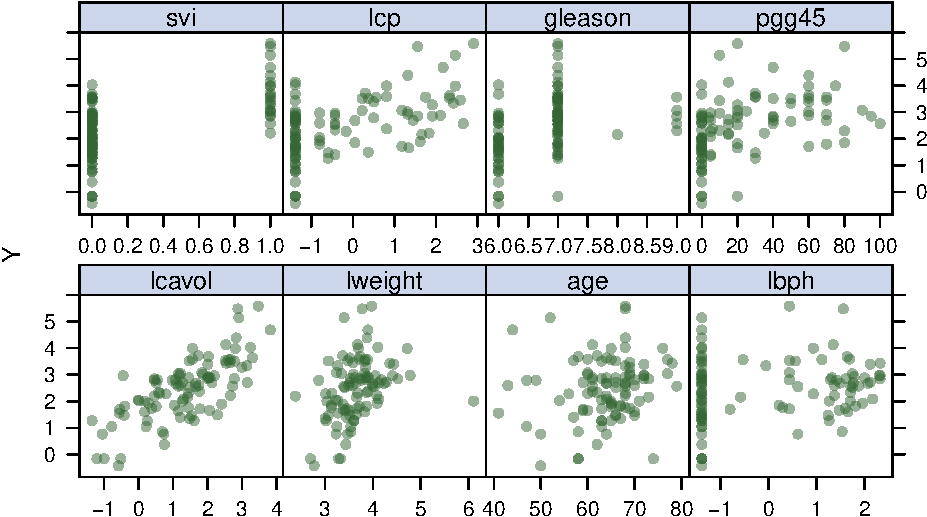
\includegraphics{HW3_files/figure-latex/unnamed-chunk-3-1.pdf}

\begin{Shaded}
\begin{Highlighting}[]
\KeywordTok{plot}\NormalTok{(Weekly}\OperatorTok{$}\NormalTok{Volume)}
\end{Highlighting}
\end{Shaded}

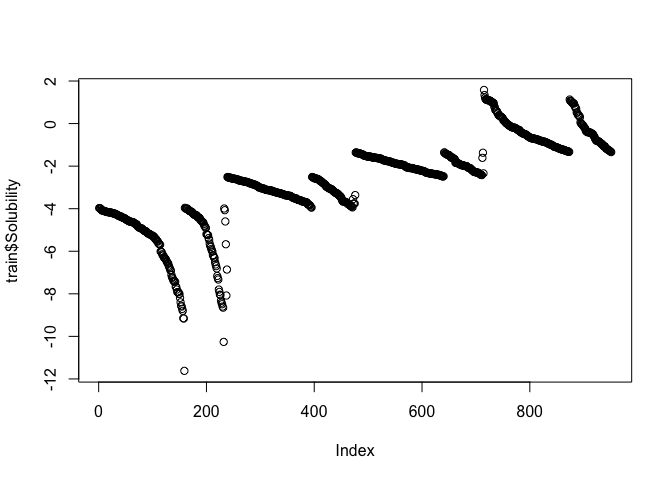
\includegraphics{HW3_files/figure-latex/unnamed-chunk-4-1.pdf}

Here we see that volume is increasing over time. Also, we see that year
is highly correlated with volume. From the graphs we can see that
lag1-lag5 are approximately normally distributed. Volume is skewed to
the right.

\begin{Shaded}
\begin{Highlighting}[]
\KeywordTok{cor}\NormalTok{(Weekly[,}\OperatorTok{-}\DecValTok{8}\NormalTok{])}
\end{Highlighting}
\end{Shaded}

\begin{verbatim}
##               Year         Lag1        Lag2        Lag3        Lag4
## Year    1.00000000 -0.032289274 -0.03339001 -0.03000649 -0.03112792
## Lag1   -0.03228927  1.000000000 -0.07485305  0.05863568 -0.07127388
## Lag2   -0.03339001 -0.074853051  1.00000000 -0.07572091  0.05838153
## Lag3   -0.03000649  0.058635682 -0.07572091  1.00000000 -0.07539587
## Lag4   -0.03112792 -0.071273876  0.05838153 -0.07539587  1.00000000
## Lag5   -0.03051910 -0.008183096 -0.07249948  0.06065717 -0.07567503
## Volume  0.84194162 -0.064951313 -0.08551314 -0.06928771 -0.06107462
##                Lag5      Volume
## Year   -0.030519101  0.84194162
## Lag1   -0.008183096 -0.06495131
## Lag2   -0.072499482 -0.08551314
## Lag3    0.060657175 -0.06928771
## Lag4   -0.075675027 -0.06107462
## Lag5    1.000000000 -0.05851741
## Volume -0.058517414  1.00000000
\end{verbatim}

\section{Question b}\label{question-b}

\begin{Shaded}
\begin{Highlighting}[]
\NormalTok{weekly =}\StringTok{ }\NormalTok{Weekly[,}\OperatorTok{-}\DecValTok{1}\NormalTok{]}
\KeywordTok{attach}\NormalTok{(weekly)}
\end{Highlighting}
\end{Shaded}

\begin{Shaded}
\begin{Highlighting}[]
\NormalTok{glm.fit =}\StringTok{ }\KeywordTok{glm}\NormalTok{(Direction }\OperatorTok{~}\StringTok{ }\NormalTok{., }\DataTypeTok{data =}\NormalTok{ weekly, }\DataTypeTok{family =}\NormalTok{ binomial)}
\KeywordTok{summary}\NormalTok{(glm.fit)}
\end{Highlighting}
\end{Shaded}

\begin{verbatim}
## 
## Call:
## glm(formula = Direction ~ ., family = binomial, data = weekly)
## 
## Deviance Residuals: 
##     Min       1Q   Median       3Q      Max  
## -1.6949  -1.2565   0.9913   1.0849   1.4579  
## 
## Coefficients:
##             Estimate Std. Error z value Pr(>|z|)   
## (Intercept)  0.26686    0.08593   3.106   0.0019 **
## Lag1        -0.04127    0.02641  -1.563   0.1181   
## Lag2         0.05844    0.02686   2.175   0.0296 * 
## Lag3        -0.01606    0.02666  -0.602   0.5469   
## Lag4        -0.02779    0.02646  -1.050   0.2937   
## Lag5        -0.01447    0.02638  -0.549   0.5833   
## Volume      -0.02274    0.03690  -0.616   0.5377   
## ---
## Signif. codes:  0 '***' 0.001 '**' 0.01 '*' 0.05 '.' 0.1 ' ' 1
## 
## (Dispersion parameter for binomial family taken to be 1)
## 
##     Null deviance: 1496.2  on 1088  degrees of freedom
## Residual deviance: 1486.4  on 1082  degrees of freedom
## AIC: 1500.4
## 
## Number of Fisher Scoring iterations: 4
\end{verbatim}

The smallest p-value here is associated with Lag2. At the 5\% level of
significance, lag2 is the only predictor that is statistically
significant.

\section{Question c}\label{question-c}

\begin{Shaded}
\begin{Highlighting}[]
\NormalTok{test.pred.prob  <-}\StringTok{ }\KeywordTok{predict}\NormalTok{(glm.fit, }\DataTypeTok{newdata =}\NormalTok{ weekly, }\DataTypeTok{type =} \StringTok{"response"}\NormalTok{)}

\NormalTok{test.pred <-}\StringTok{ }\KeywordTok{rep}\NormalTok{(}\StringTok{"Down"}\NormalTok{, }\KeywordTok{length}\NormalTok{(test.pred.prob))}

\NormalTok{test.pred[test.pred.prob }\OperatorTok{>}\StringTok{ }\FloatTok{0.5}\NormalTok{] <-}\StringTok{ "Up"}
\end{Highlighting}
\end{Shaded}

\begin{Shaded}
\begin{Highlighting}[]
\KeywordTok{confusionMatrix}\NormalTok{(}\DataTypeTok{data =} \KeywordTok{as.factor}\NormalTok{(test.pred),}
                \DataTypeTok{reference =}\NormalTok{ weekly}\OperatorTok{$}\NormalTok{Direction,}
                \DataTypeTok{positive =} \StringTok{"Up"}\NormalTok{)}
\end{Highlighting}
\end{Shaded}

\begin{verbatim}
## Confusion Matrix and Statistics
## 
##           Reference
## Prediction Down  Up
##       Down   54  48
##       Up    430 557
##                                          
##                Accuracy : 0.5611         
##                  95% CI : (0.531, 0.5908)
##     No Information Rate : 0.5556         
##     P-Value [Acc > NIR] : 0.369          
##                                          
##                   Kappa : 0.035          
##  Mcnemar's Test P-Value : <2e-16         
##                                          
##             Sensitivity : 0.9207         
##             Specificity : 0.1116         
##          Pos Pred Value : 0.5643         
##          Neg Pred Value : 0.5294         
##              Prevalence : 0.5556         
##          Detection Rate : 0.5115         
##    Detection Prevalence : 0.9063         
##       Balanced Accuracy : 0.5161         
##                                          
##        'Positive' Class : Up             
## 
\end{verbatim}

\begin{Shaded}
\begin{Highlighting}[]
\KeywordTok{mean}\NormalTok{(test.pred }\OperatorTok{==}\StringTok{ }\NormalTok{weekly}\OperatorTok{$}\NormalTok{Direction)}
\end{Highlighting}
\end{Shaded}

\begin{verbatim}
## [1] 0.5610652
\end{verbatim}

The diagonal elements of the confusion matrix indicate correct
predictions, while the off-diagonals represent incorrect predictions.
Hence our model correctly predicted that the market would go up on 124
weeks and that it would go down on 18 days, for a total of 54 + 557 =
611 correct predictions. We also see that the model predicts 56.1\% of
the time.

\section{Question d}\label{question-d}

\begin{Shaded}
\begin{Highlighting}[]
\NormalTok{roc.glm <-}\StringTok{ }\KeywordTok{roc}\NormalTok{(weekly}\OperatorTok{$}\NormalTok{Direction, test.pred.prob)}

\KeywordTok{plot}\NormalTok{(roc.glm, }\DataTypeTok{legacy.axes =} \OtherTok{TRUE}\NormalTok{, }\DataTypeTok{print.auc =} \OtherTok{TRUE}\NormalTok{)}
\KeywordTok{plot}\NormalTok{(}\KeywordTok{smooth}\NormalTok{(roc.glm), }\DataTypeTok{col =} \DecValTok{4}\NormalTok{, }\DataTypeTok{add =} \OtherTok{TRUE}\NormalTok{)}
\end{Highlighting}
\end{Shaded}

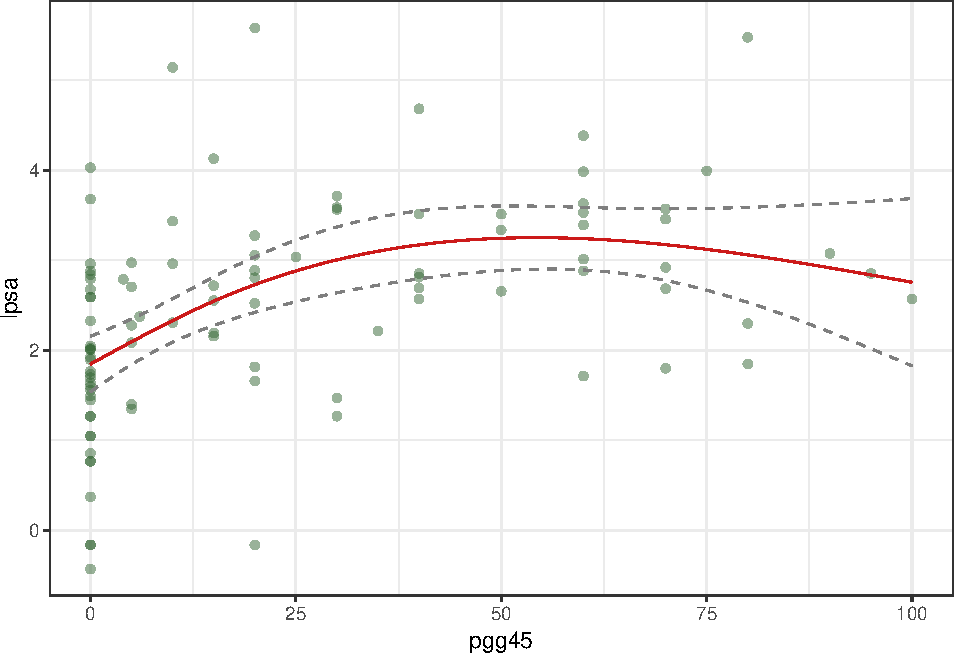
\includegraphics{HW3_files/figure-latex/unnamed-chunk-10-1.pdf}

The AUC is 0.554.

\section{Question e}\label{question-e}

\begin{Shaded}
\begin{Highlighting}[]
\NormalTok{train =}\StringTok{ }\NormalTok{(Weekly}\OperatorTok{$}\NormalTok{Year }\OperatorTok{<}\StringTok{ }\DecValTok{2009}\NormalTok{)}
\NormalTok{weekly_}\DecValTok{2008}\NormalTok{ =}\StringTok{ }\NormalTok{weekly[}\OperatorTok{!}\NormalTok{train,}\DecValTok{1}\OperatorTok{:}\DecValTok{2}\NormalTok{]}
\NormalTok{Direction_}\DecValTok{2008}\NormalTok{ =}\StringTok{ }\NormalTok{weekly}\OperatorTok{$}\NormalTok{Direction[}\OperatorTok{!}\NormalTok{train]}
\end{Highlighting}
\end{Shaded}

\begin{Shaded}
\begin{Highlighting}[]
\NormalTok{glm.fit =}\StringTok{ }\KeywordTok{glm}\NormalTok{(Direction }\OperatorTok{~}\StringTok{ }\NormalTok{Lag1 }\OperatorTok{+}\StringTok{ }\NormalTok{Lag2, }\DataTypeTok{data =}\NormalTok{ weekly, }\DataTypeTok{family =}\NormalTok{ binomial, }\DataTypeTok{subset =}\NormalTok{ train)}
\NormalTok{glm.probs =}\StringTok{ }\KeywordTok{predict}\NormalTok{(glm.fit, weekly_}\DecValTok{2008}\NormalTok{, }\DataTypeTok{type =} \StringTok{"response"}\NormalTok{)}

\NormalTok{test.pred <-}\StringTok{ }\KeywordTok{rep}\NormalTok{(}\StringTok{"Down"}\NormalTok{, }\KeywordTok{length}\NormalTok{(glm.probs))}
\NormalTok{test.pred[glm.probs }\OperatorTok{>}\StringTok{ }\FloatTok{0.5}\NormalTok{] <-}\StringTok{ "Up"}
\end{Highlighting}
\end{Shaded}

\begin{Shaded}
\begin{Highlighting}[]
\NormalTok{roc.glm <-}\StringTok{ }\KeywordTok{roc}\NormalTok{(Direction_}\DecValTok{2008}\NormalTok{, glm.probs)}
\KeywordTok{plot}\NormalTok{(roc.glm, }\DataTypeTok{legacy.axes =} \OtherTok{TRUE}\NormalTok{, }\DataTypeTok{print.auc =} \OtherTok{TRUE}\NormalTok{)}
\KeywordTok{plot}\NormalTok{(}\KeywordTok{smooth}\NormalTok{(roc.glm), }\DataTypeTok{col =} \DecValTok{4}\NormalTok{, }\DataTypeTok{add =} \OtherTok{TRUE}\NormalTok{)}
\end{Highlighting}
\end{Shaded}

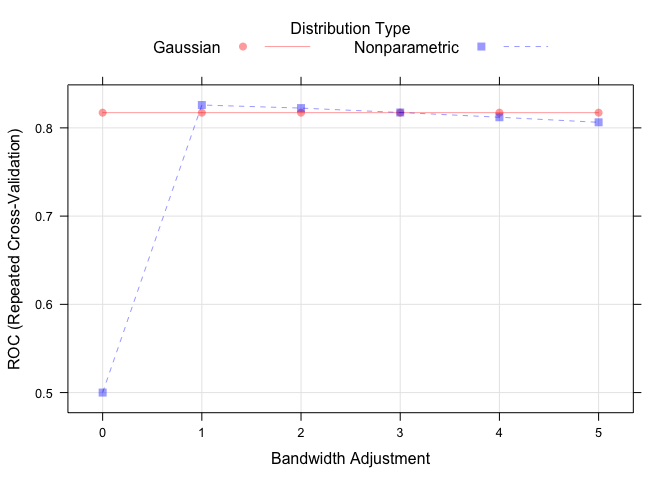
\includegraphics{HW3_files/figure-latex/unnamed-chunk-13-1.pdf}

The AUC for the logistic regression model with just Lag1 and Lag2 is
0.557.

\section{Question f}\label{question-f}

\subsection{LDA}\label{lda}

\begin{Shaded}
\begin{Highlighting}[]
\NormalTok{lda.fit <-}\StringTok{ }\KeywordTok{lda}\NormalTok{(Direction }\OperatorTok{~}\StringTok{ }\NormalTok{Lag1 }\OperatorTok{+}\StringTok{ }\NormalTok{Lag2, }\DataTypeTok{data =}\NormalTok{ weekly, }\DataTypeTok{subset =}\NormalTok{ train)}
\KeywordTok{plot}\NormalTok{(lda.fit)}
\end{Highlighting}
\end{Shaded}

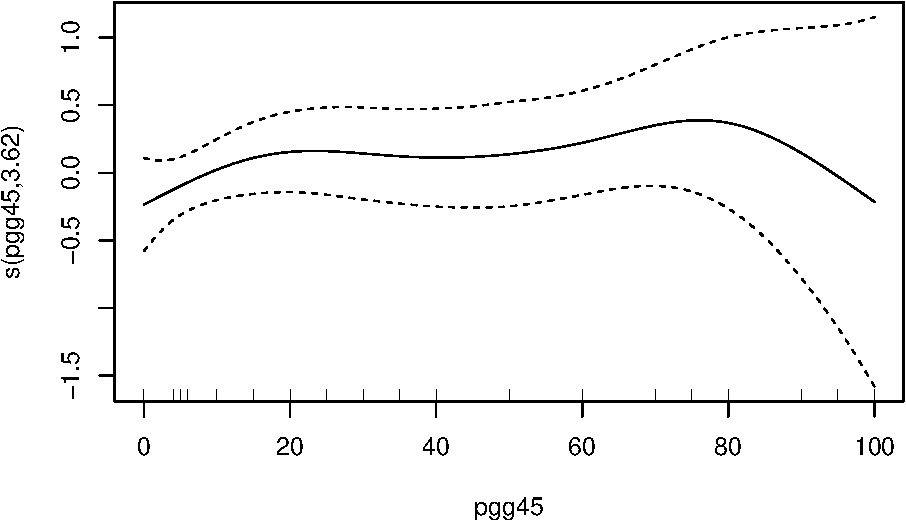
\includegraphics{HW3_files/figure-latex/unnamed-chunk-14-1.pdf}

Evaluating the test set performance using ROC.

\begin{Shaded}
\begin{Highlighting}[]
\NormalTok{lda.pred <-}\StringTok{ }\KeywordTok{predict}\NormalTok{(lda.fit, }\DataTypeTok{newdata =}\NormalTok{ weekly_}\DecValTok{2008}\NormalTok{)}

\NormalTok{roc.lda <-}\StringTok{ }\KeywordTok{roc}\NormalTok{(Direction_}\DecValTok{2008}\NormalTok{, lda.pred}\OperatorTok{$}\NormalTok{posterior[,}\DecValTok{2}\NormalTok{], }
               \DataTypeTok{levels =} \KeywordTok{c}\NormalTok{(}\StringTok{"Down"}\NormalTok{, }\StringTok{"Up"}\NormalTok{))}
\KeywordTok{plot}\NormalTok{(roc.lda, }\DataTypeTok{legacy.axes =} \OtherTok{TRUE}\NormalTok{, }\DataTypeTok{print.auc =} \OtherTok{TRUE}\NormalTok{)}
\end{Highlighting}
\end{Shaded}

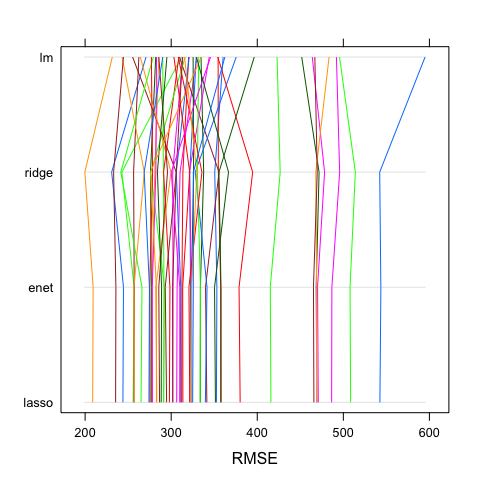
\includegraphics{HW3_files/figure-latex/unnamed-chunk-15-1.pdf}

The AUC for LDA is 0.557.

\subsection{QDA}\label{qda}

\begin{Shaded}
\begin{Highlighting}[]
\CommentTok{# use qda() in MASS}
\NormalTok{qda.fit <-}\StringTok{ }\KeywordTok{qda}\NormalTok{(Direction }\OperatorTok{~}\StringTok{ }\NormalTok{Lag1 }\OperatorTok{+}\StringTok{ }\NormalTok{Lag2, }\DataTypeTok{data =}\NormalTok{ weekly, }\DataTypeTok{subset =}\NormalTok{ train)}

\NormalTok{qda.pred <-}\StringTok{ }\KeywordTok{predict}\NormalTok{(qda.fit, }\DataTypeTok{newdata =}\NormalTok{ weekly_}\DecValTok{2008}\NormalTok{)}

\NormalTok{roc.qda <-}\StringTok{ }\KeywordTok{roc}\NormalTok{(Direction_}\DecValTok{2008}\NormalTok{, qda.pred}\OperatorTok{$}\NormalTok{posterior[,}\DecValTok{2}\NormalTok{], }
               \DataTypeTok{levels =} \KeywordTok{c}\NormalTok{(}\StringTok{"Down"}\NormalTok{, }\StringTok{"Up"}\NormalTok{))}
\KeywordTok{plot}\NormalTok{(roc.qda, }\DataTypeTok{legacy.axes =} \OtherTok{TRUE}\NormalTok{, }\DataTypeTok{print.auc =} \OtherTok{TRUE}\NormalTok{)}
\end{Highlighting}
\end{Shaded}

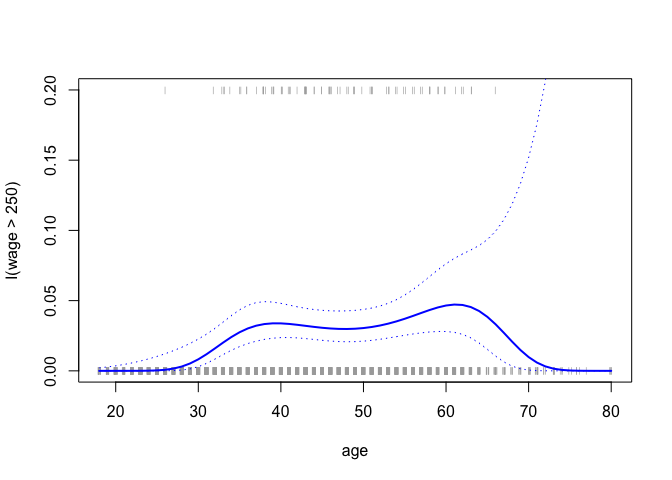
\includegraphics{HW3_files/figure-latex/unnamed-chunk-16-1.pdf}

The AUC for QDA is 0.529.

\section{Question g}\label{question-g}

\begin{Shaded}
\begin{Highlighting}[]
\NormalTok{ctrl <-}\StringTok{ }\KeywordTok{trainControl}\NormalTok{(}\DataTypeTok{method =} \StringTok{"repeatedcv"}\NormalTok{,}
                     \DataTypeTok{repeats =} \DecValTok{5}\NormalTok{,}
                     \DataTypeTok{summaryFunction =}\NormalTok{ twoClassSummary,}
                     \DataTypeTok{classProbs =} \OtherTok{TRUE}\NormalTok{)}

\KeywordTok{set.seed}\NormalTok{(}\DecValTok{1}\NormalTok{)}
\NormalTok{model.knn <-}\StringTok{ }\KeywordTok{train}\NormalTok{(}\DataTypeTok{x =}\NormalTok{ weekly[train,}\DecValTok{1}\OperatorTok{:}\DecValTok{2}\NormalTok{],}
                   \DataTypeTok{y =}\NormalTok{ weekly}\OperatorTok{$}\NormalTok{Direction[train],}
                   \DataTypeTok{method =} \StringTok{"knn"}\NormalTok{,}
                   \DataTypeTok{preProcess =} \KeywordTok{c}\NormalTok{(}\StringTok{"center"}\NormalTok{,}\StringTok{"scale"}\NormalTok{),}
                   \DataTypeTok{tuneGrid =} \KeywordTok{data.frame}\NormalTok{(}\DataTypeTok{k =} \KeywordTok{seq}\NormalTok{(}\DecValTok{1}\NormalTok{, }\DecValTok{50}\NormalTok{, }\DataTypeTok{by =} \DecValTok{1}\NormalTok{)),}
                   \DataTypeTok{trControl =}\NormalTok{ ctrl,}
                   \DataTypeTok{metric =} \StringTok{'ROC'}\NormalTok{)}

\KeywordTok{ggplot}\NormalTok{(model.knn)}
\end{Highlighting}
\end{Shaded}

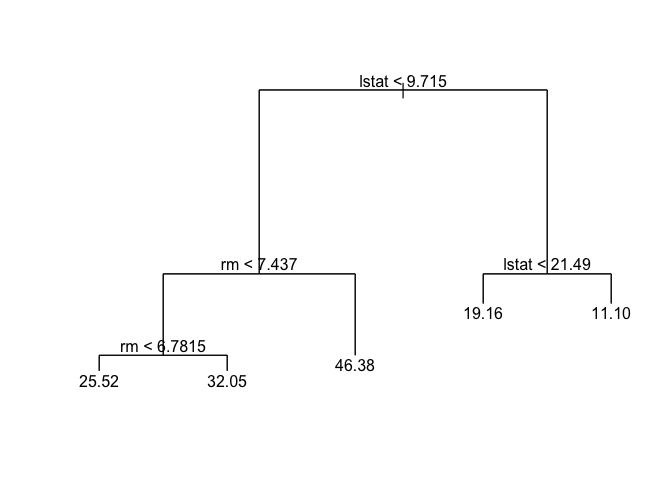
\includegraphics{HW3_files/figure-latex/unnamed-chunk-17-1.pdf}

\begin{Shaded}
\begin{Highlighting}[]
\NormalTok{knn.pred <-}\StringTok{ }\KeywordTok{predict}\NormalTok{(model.knn, }\DataTypeTok{newdata =}\NormalTok{ weekly_}\DecValTok{2008}\NormalTok{, }\DataTypeTok{type =} \StringTok{"prob"}\NormalTok{)[,}\DecValTok{2}\NormalTok{]}

\NormalTok{roc.knn <-}\StringTok{ }\KeywordTok{roc}\NormalTok{(Direction_}\DecValTok{2008}\NormalTok{, knn.pred)}
\KeywordTok{plot}\NormalTok{(roc.knn, }\DataTypeTok{legacy.axes =} \OtherTok{TRUE}\NormalTok{, }\DataTypeTok{print.auc =} \OtherTok{TRUE}\NormalTok{)}
\end{Highlighting}
\end{Shaded}

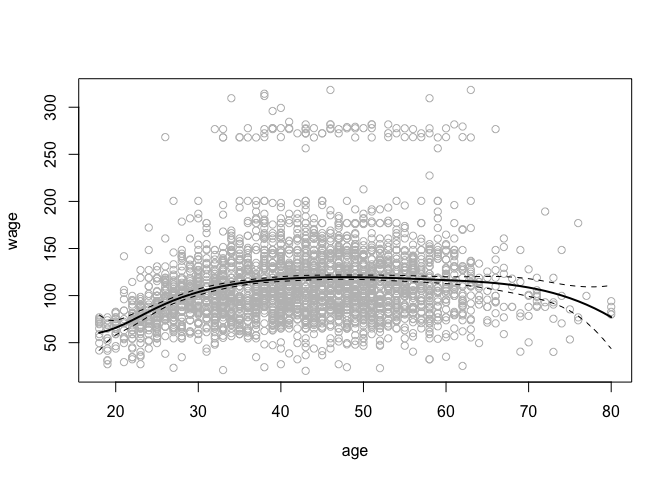
\includegraphics{HW3_files/figure-latex/unnamed-chunk-18-1.pdf}

AUC for the K Nearest Neighbor is 0.545.

At first glance, it appears that the logistic regression model is
working a little better than random guessing. However, this result is
misleading because we trained and tested the model on the same set
observations. In other words, 100 − 56.10652 = 43.893 \% is the training
error rate. The training error rate is often overly optimistic and it
tends to underestimate the test error rate.

In order to better assess the accuracy of the logistic regression model
in this setting, we fit the model using part of the data, and then
examined how well it predicts the held out data. This will yield a more
realistic error rate.

The AUC provides a good way of comparing the perfomance of a classifier
based of different cut off points. We expect the AUC of the held out
data to be less or similar compared to the full dataset. We see that the
AUC of the logistic model with the full data set is 0.557 and the AUC on
the held out data is 0.554. AUC for the K Nearest Neighbor is 0.545. The
best tune K is 7. The AUC for QDA is 0.529 and for LDA is 0.557. They
all perform similarly because it is difficult to predict stock price
changes simply based on the previous days (lag1 and lag2). Also, using
the only lag1 and lag2, the p values using logistic regression are not
significant for the subset of our data suggesting that lag1 and lag2 may
not be associated with the direction. Predictors that are not associated
with the outcome contribute to an increase in variance without
corresponding decrease in the bias therefore perform inadequated when
used for prediction.


\end{document}
